\documentclass{standalone}
\begin{document}
\subsection{Prediction of Response}

The prediction of response is based on the Tumor Regression Grade (TRG) which indicates the degree of response to neo-adjuvant therapy\cite{tesicoppola}. TRG ranges from 0 to 5, resulting in a different response. Lower is the TRG higher the response. 
\\
To obtain the prediction of response, a custom Classifier has been made.
The classifier consists of a \textit{pipeline} object which is made by the given estimators from the \textsc{Scikit-learn} library: 
\begin{itemize}
    \item $\mathtt{StandardScaler}$: to standardize the data
    \item $\mathtt{PCA}$: to perform PCA as described previously
    \item $\mathtt{SVC}$: Support Vector Classifier
\end{itemize}
Unfortunately, not for every patient, the TRG was registered in the clinical database provided by the IRCCS Sant'Orsola-Malpighi Policlinic, so patients without it were excluded from the analysis.
In the end, the total number of patients was 32. 
Moreover, since the lack of much data TRG values were binarized into two main classes: 0 and 1.
Class 0 means a complete response to the neo-adjuvant chemo-radiotherapy (TRG values $ \in [0, \: 1])$ while class 1 means a moderate response (TRG values $ \in [2, \: 3])$ .
In Figure \ref{classesdistrib} you can see the distribution of the two classes that are not equally distributed.\\
The Classifier model was then trained with Cross-validation (using 10 folds) to avoid the presence of \textit{bias} during the split into training and test set.
The Matthews correlation coefficient (MCC) was used as a  measure of the quality of classifications between the true label and the model prediction. 
It takes into account true and false positives and negatives and is generally regarded as a balanced measure that can be used even if the classes are of very different sizes. 
The MCC is a correlation coefficient ranging between -1 and +1. 
A coefficient of +1 represents a perfect prediction, 0 is an average random prediction, and -1 is an inverse prediction.
In particular, for Cross-validation it was used the $\mathtt{StratifiedKfold}$ (i.e. object that provides train/test indices to split data in train/test sets) from \textsc{Scikit-learn} that gives the median value, $median = 0.55$, of the MCC distribution (Figure \ref{MCC}), obtained after 500 simulations.

\begin{figure}[ht]

    \centering
    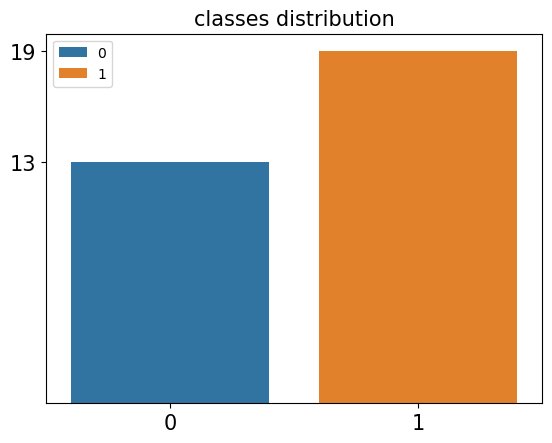
\includegraphics[width=0.65\textwidth]{../images/classesdistrib.png}

    \caption{Distribution of the classes. Class 0 means a complete response to the neo-adjuvant chemo-radiotherapy (TRG values $ \in [0, \: 1])$ while class 1 means a moderate response (TRG values $ \in [2, \: 3])$ }
    \label{classesdistrib}
    
    \end{figure}

    \begin{figure}[ht]

        \centering
        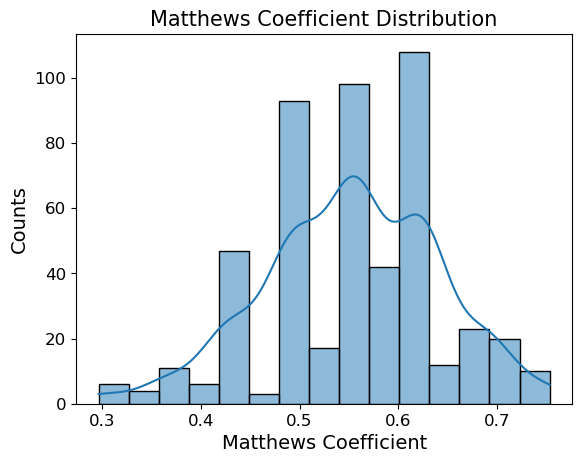
\includegraphics[width=0.65\textwidth]{../images/MCC.png}
    
        \caption{Matthews Correlation coefficient distribution. Obtained after 500 simulations, changing the $\mathtt{random\_state}$ (i.e. the randomness) of the $\mathtt{StratifiedKfold}$ (i.e. object that provides train/test indices to split data in train/test sets) from \textsc{Scikit-learn}.}
        \label{MCC}
        
        \end{figure}


\end{document}